\chapter{Propositional Logic}
\markright{Chap. \ref{ch:SL}: Propositional Logic}
\label{ch:SL}


In Part \ref{part:cat_logic}, we introduced a system of logic that dealt with categorical statements, statements like ``All people are mortal'' or ``Some dogs have  fleas.'' The system developed there was somewhat formal, because it replaced some of the contents of ordinary English sentences with abstract symbols. In Part \ref{part:sent_logic}, we go the rest of the way, and replace all of ordinary English with abstract symbols, thus creating a fully artificial language. In the previous system, capital letters like $S$ and $P$ stood for categories, like ``dogs'' or ``things that have fleas.'' In the new system individual letters will stand for whole sentences, like ``Tom wants to go to the bookstore'' or ``The sky is blue.'' Because individual letters stand for sentences this kind of system is known as \textit{sentential logic}, a term which we will be able to precisely define on page \pageref{def:sentential_logic}. We will call the specific version of sentential logic we will be developing SL.

\section{Sentence Letters}


\newglossaryentry{sentence letter}
{
name=sentence letter,
description={A single capital letter, used in SL to represent a statement.}
}

The most basic unit in our formal language SL is an individual capital letter---$A, B, C, D$, etc. These letters, called \textsc{\glspl{sentence letter}}, \label{def:sentence_letter} are used to represent individual statements. Remember in section \ref{def:statement}, we defined a statement as some bit of language that can be true or false, and listed all kinds of things that count as statements in English, from ``\emph{Tyrannosaurus rex} went extinct 65 million years ago'' to ``Lady Gaga is pretty.'' In SL, all these statements are reduced to single capital letters.

\newglossaryentry{translation key}
{
name=translation key,
description={A list that assigns English phrases or sentences to variable names. Also called a ``symbolization key''  or simply a ``dictionary.''}
}

Considered only as a symbol of SL, the letter $A$ could mean any statement.

So when translating from English into SL, it is important to provide a \gls{translation key}\label{def:translation_key}. Previously, we used translation keys to say assign the variables $S$, $M$, and $P$ to terms. (See page \pageref{def:translation_key}.) Now we will use them to assign sentences to sentence letters.

In order to specify what we mean, we need to provide a key saying what the sentence letters represent. We will call a list that assigns English phrases or sentences to variable names a \textsc{\gls{translation key}}.\label{def:translation_key} These are sometimes also called ``symbolization keys'' or simply just ``dictionaries.''

Consider this argument (recall that the portion of the passage in italics establishes the context, and is not part of the passage):

\begin{quotation}
\noindent \textit{A teacher is looking to see who has come to class} There is an apple on the desk. If there is an apple on the desk, then Jenny made it to class. Therefore, Jenny made it to class.
\end{quotation}

In canonical form, the argument would look like this:

\begin{kormanize}
\premise{There is an apple on the desk.}
\premise{If there is an apple on the desk, then Jenny made it to class.}
\conclusion{Jenny made it to class.}
\end{kormanize}

A good symbolization key for this passage would look like this:

\begin{description}
\item[A:]There is an apple on the desk.
\item[B:]Jenny made it to class.
\end{description}

Why do the symbolization key this way? The argument we are looking at is obviously valid in English. In symbolizing it, we want to preserve the structure of the argument that makes it valid. We could have made each sentence in the original argument into its own letter. Then the symbolization key would look like this:

\begin{description}
\item[A:]There is an apple on the desk.
\item[B:]If there is an apple on the desk, then Jenny made it to class.
\item[C:]Jenny made it to class.
\end{description}

But that would mean the argument would look like this:

\begin{kormanize}
\premise{$A$}
\premise{$B$}
\conclusion{$C$}
\end{kormanize}

There is no necessary connection between some sentence $A$, which could be any statement, and some other sentences $B$ and $C$, which could also be anything. The structure of the argument has been completely lost in this translation.

The important thing about the argument is that the second premise is not merely \emph{any} statement, logically divorced from the other statement in the argument. The second premise contains the first premise and the conclusion \emph{as parts}. Our original symbolization key allows us to write the argument like this.

\begin{kormanize}
\premise{$A$}
\premise{If $A$, then $B$.}
\conclusion{$B$}
\end{kormanize}

This preserves the structure of the argument that makes it valid, but it still makes use of the English expression ``If$\ldots$ then$\ldots$.'' Although we ultimately want to replace all of the English expressions with logical notation, this is a good start.

\newglossaryentry{atomic sentence}
{
name=atomic sentence,
description={A sentence that does not have any sentences as proper parts.}
}

The individual sentence letters in SL are called atomic sentences, because they are the basic building blocks out of which more complex sentences can be built. We can identify atomic sentences in English as well. An \textsc{\gls{atomic sentence}} \label{def:atomic_sentence} is one that cannot be broken into parts that are themselves sentences. ``There is an apple on the desk'' is an atomic sentence in English, because you can't find any proper part of it that forms a complete sentence. For instance ``an apple on the desk'' is a noun phrase, not a complete sentence. Similarly ``on the desk'' is a prepositional phrase, and not a sentence, and ``is an'' is not any kind of phrase at all. This is what you will find no matter how you divide ``There is an apple on the desk.'' On the other hand you can find two proper parts of ``If there is an apple on the desk, then Jenny made it to class'' that are complete sentences: ``There is an apple on the desk'' and ``Jenny made it to class.'' As a general rule, we will want to use atomic sentences in SL (that is, the sentence letters) to represent atomic sentences in English. Otherwise, we will lose some of the logical structure of the English sentence, as we have just seen.

There are only 26 letters of the alphabet, but there is no logical limit to the number of atomic sentences. We can use the same letter to symbolize different atomic sentences by adding a subscript, a small number written after the letter. We could have a symbolization key that looks like this:

\begin{description}
\item[A$_1$:] The apple is under the armoire.
\item[A$_2$:] Arguments in SL always contain atomic sentences.
\item[A$_3$:] Adam Ant is taking an airplane from Anchorage to Albany.
\item[$\vdots$]
\item[A$_{294}$:] Alliteration angers otherwise affable astronauts.
\end{description}

Keep in mind that each of these is a different sentence letter. When there are subscripts in the symbolization key, it is important to keep track of them.

\section{Sentential Connectives}

The previous section introduced the basic elements of SL, the sentence letters. But when we were looking at the argument involving Jenny and the apple, we saw that the best way to write a dictionary for the argument left the words ``if'' and ``then'' in English. In this section we will introduce ways to connect the sentence letters together that will allow us to form a complete artificial language.

\newglossaryentry{sentential connective}
{
name=sentential connective,
description={A logical operator in SL used to combine sentence letters into larger sentences.}
}

\newglossaryentry{logical constant}
{
name=logical constant,
description={A symbol whose meaning is fixed by a formal language. Sometimes these are just called ``logical symbols.'' They are contrasted with \textsc{non-logical symbols}.}
}

\newglossaryentry{nonlogical symbol}
{
name=nonlogical symbol,
description={A symbol whose meaning is not fixed by a formal language.}
}

The symbols used to connect sentence letters are called \textsc{\glspl{sentential connective}} \label{def:sentential_connective}, naturally enough. SL uses five sentential connectives: $\land$, $\lor$, $\lnot$, $\onlyif$, and $\iff$. To write the sentence about Jenny and the apple we use the symbol ``$\onlyif$.'' Using the dictionary above, ``If there is an apple on the desk, then Jenny made it to class'' becomes $A \onlyif B$. Table \ref{table:sentential_connectives} summarizes the meaning of the five sentential connectives.

The sentential connectives are a kind of \textsc{\gls{logical constant}},\label{def:logical_constant} because their meaning is fixed by the formal language that we have chosen. The other logical constants in SL are the parentheses. These are the things we cannot change in the symbolization key. The sentence letters, by contrast, are \textsc{\glspl{nonlogical symbol}}, \label{def:nonlogical_symbol} because their meaning can change as we change the symbolization key. We can decide that $A$ stands for ``Arthur is an aardvark'' in one translation key and ``Apu is an anthropologist'' in the next. But we can't say that the  the $\lnot$ symbol will mean ``not'' in one argument and ``perhaps'' in another.

The sections below describe each connective in more detail.

\begin{table}
\begin{tabu}{X[1,c] X[3,c] X[3,c]}
\textbf{Symbol} & \textbf{What it is called} & \textbf{What it means}\\
$\lnot$   & negation&      ``It is not the case that$\ldots$''\\
$\land$   & conjunction&   ``Both $\ldots$\ and $\ldots$''\\
$\lor$    & disjunction&   ``Either $\ldots$\ or $\ldots$''\\
$\onlyif$ & conditional&   ``If $\ldots$\ then $\ldots$''\\
$\iff$    & biconditional& ``$\ldots$ if and only if $\ldots$''\\
\end{tabu}
\caption{The Sentential Connectives.}
\label{table:sentential_connectives}
\end{table}

\section{Negation}
Consider how we might symbolize these sentences:

\begin{enumerate}
\item Mary is in Barcelona. \label{itm:not1}
\item Mary is not in Barcelona. \label{itm:not2}
\item Mary is somewhere other than Barcelona. \label{itm:not3}
\end{enumerate}

In order to symbolize sentence \ref{itm:not1}, we will need one sentence letter. We can provide a symbolization key:

\begin{description}
\item[B:]Mary is in Barcelona.
\end{description}

Note that here we are giving $B$ a different interpretation than we did in the previous section. The symbolization key only specifies what $B$ means \emph{in a specific context}. It is vital that we continue to use this meaning of $B$ so long as we are talking about Mary and Barcelona. Later, when we are symbolizing different sentences, we can write a new symbolization key and use $B$ to mean something else.

\newglossaryentry{negation}
{
name=negation,
description={The symbol \(\lnot\), used to represent words and phrases that function like the English word ``not''.}
}

Now, sentence \ref{itm:not1} is simply $B$. Sentence \ref{itm:not2} is obviously related to sentence \ref{itm:not1}: it is basically \ref{itm:not1} with a ``not'' added. We could put the sentence partly our symbolic language by writing ``Not $B$.'' This means we do not want to introduce a different sentence letter for \ref{itm:not2}. We just need a new symbol for the ``not'' part. Let's use the symbol `$\lnot$,' which we will call \textsc{\gls{negation}}. \label{def:negation} Now we can translate `Not $B$' to $\lnot B$.

Sentence \ref{itm:not3} is about whether or not Mary is in Barcelona, but it does not contain the word ``not.'' Nevertheless, it is obviously logically equivalent to sentence \ref{itm:not2}. They both say that if you are looking for Mary, you shouldn't look in Barcelona. Remember that in section \ref{def:logical_equivalence}, we said that two sentences in English are logically equivalent if they always have the same truth value. For our purposes, this means that they basically say the same thing. It is clear then that \ref{itm:not2} and \ref{itm:not3} are logically equivalent, so we can translate them both as $\lnot B$.

Consider these further examples:
\begin{enumerate}
\item The widget can be replaced if it breaks. \label{itm:not4}
\item The widget is irreplaceable. \label{itm:not5}
\item The widget is not irreplaceable. \label{itm:not5b}
\end{enumerate}

If we let $R$ mean ``The widget is replaceable'', then sentence \ref{itm:not4} can be translated as $R$. Sentence \ref{itm:not5} means the opposite of sentence \ref{itm:not4}, so we can translate it $\lnot R$. Sentence \ref{itm:not5b} adds another negation to sentence \ref{itm:not5}. We know, as competent English speakers, that the two negations cancel each other out, so that sentence \ref{itm:not5b} is equivalent to sentence \ref{itm:not4}. But the fact that two negations cancel each other out is a part of the logic of English that we actually want to capture with our formal language SL.
So we will represent the two negations in sentence \ref{itm:not5b} as two negations in SL: $\lnot\lnot R$. We will now have to be sure that in SL the sentences $R$ and $\lnot \lnot R$ mean the same thing.

As the above examples begin to indicate, English has all kinds of ways to negate a sentence.  Sometimes we use an explicit ``not.'' Sometimes we use a prefix like the ``ir-'' in ``irreplaceable.'' SL has just one way to form a negation: slap a $\lnot$ in front of the sentence. There is an English expression, however, that always occurs in the same place in an English sentence as the $\lnot$ occurs in the sentence SL. The English phrase is ``It is not the case that.'' Although this phrase sounds awkward, it always occurs in front of the sentence it is negating, just as the symbol $\lnot$ does. This makes it useful in translating sentences from SL back into English. $\lnot R$ can be translated ``it is not the case that this widget is replaceable.'' In the earlier example, $\lnot B$ can be translated ``It is not the case that Mary is in Barcelona.''

\marginnote{
A sentence can be symbolized as $\lnot\mathcal{A}$ can always be paraphrased in English as ``It is not the case that $\mathcal{A}$.''
}

Sometimes negations in English do not function as neatly as the $\lnot$ does in SL, because two things aren't perfect opposites. Consider these sentences:

\begin{enumerate}
\item Elliott is happy. \label{itm:not6}
\item Elliott is unhappy. \label{itm:not7}
\end{enumerate}


If we let $H$ mean ``Elliot is happy'', then we can symbolize sentence \ref{itm:not6} as $H$, but does \ref{itm:not7} really mean the same thing as $\lnot H$? Saying ``Elliott is unhappy'' indicates that Elliott is actively sad. But $\lnot H$ can be paraphrase as simply ``It is not the case that Elliott is happy,'' which might merely mean that Elliott is just feeling neutral. As we saw on page \pageref{def:bivalent}, the logics we discuss in this textbook are \emph{bivalent}. Statements are only either true or false. Everything is in black and white, and issues like Elliott's fine gradations in mood cannot be directly represented in our system. So in SL, sentences \ref{itm:not6} and  \ref{itm:not7} would generally be represented by separate sentence letters.

One way of capturing the meaning of a sentential connective is to make a table which shows how the connective changes the meaning of the sentences it is applied to. The negation simply reverses the truth value of any sentence it is put in front of. For any sentence $\mathcal{A}$: If $\mathcal{A}$ is true, then $\lnot\mathcal{A}$ is false. If $\lnot\mathcal{A}$ is true, then $\mathcal{A}$ is false. Using T for true and F for false, we can summarize this in a \emph{characteristic truth table} for negation:

\begin{table}
\begin{tabular}{c|c}
$\mathcal{A}$ & $\lnot\mathcal{A}$\\
\hline
T & F\\
F & T
\end{tabular}
\end{table}

We will discuss truth tables at greater length in the next chapter.

%%%%%%%%%%%%%%%%%% 2.2.2 Conjunction

\section{Conjunction}
Consider these sentences:
\begin{enumerate}
\item Alex is athletic. \label{itm:and1}
\item Barbara is athletic. \label{itm:and2}
\item Alex is athletic, and Barbara is also athletic. \label{itm:and3}
\end{enumerate}

We will need separate sentence letters for \ref{itm:and1} and \ref{itm:and2}, so we define this symbolization key:

\begin{description}
\item[A:] Alex is athletic.
\item[B:] Barbara is athletic.
\end{description}

\newglossaryentry{conjunction}
{
name=conjunction,
description={The symbol \(\land\), used to represent words and phrases that function like the English word ``and.''}
}

\newglossaryentry{conjunct}
{
name=conjunct,
description={A sentence joined to another by a conjunction.}
}

Sentence \ref{itm:and1} can be symbolized as $A$. Sentence \ref{itm:and2} can be symbolized as $B$. Sentence \ref{itm:and3} can be paraphrased as ``$A$ and $B$.'' In order to fully symbolize this sentence, we need another symbol.
We will use $\land$. We translate ``$A$ and $B$'' as $A\land B$. The logical connective $\land$ is called the \textsc{\gls{conjunction}}, \label{def:conjunction} and $A$ and $B$ are each called \textsc{\glspl{conjunct}}. \label{def:conjunct}

Notice that we make no attempt to symbolize ``also'' in sentence \ref{itm:and3}. Words like ``both'' and ``also'' function to draw our attention to the fact that two things are being conjoined. They are not doing any further logical work, so we do not need to represent them in SL.

Some more examples:
\begin{enumerate}
\item Barbara is athletic and energetic. \label{itm:and4}
\item Barbara and Alex are both athletic. \label{itm:and5}
\item Although Barbara is energetic, she is not athletic. \label{itm:and6}
\item Barbara is athletic, but Alex is more athletic than she is. \label{itm:and7}
\end{enumerate}

Sentence \ref{itm:and4} is obviously a conjunction. The sentence says two things about Barbara, so in English it is permissible to refer to Barbara only once. It might be tempting to try this when translating the argument: Since $B$ means ``Barbara is athletic'', one might paraphrase the sentences as ``$B$ and energetic.'' This would be a mistake. Once we translate part of a sentence as $B$, any further structure is lost. $B$ is an atomic sentence; it is nothing more than true or false. Conversely, ``energetic'' is not a sentence; on its own it is neither true nor false. We should instead paraphrase the sentence as ``$B$ and Barbara is energetic.'' Now we need to add a sentence letter to the symbolization key. Let $E$ mean ``Barbara is energetic.'' Now the sentence can be translated as $B \land E$.
\marginnote{
A sentence can be symbolized as $\mathcal{A} \land \mathcal{B}$ if it can be paraphrased in English as `Both $\mathcal{A}$, and $\mathcal{B}$.' Each of the conjuncts must be a sentence.
}

Sentence \ref{itm:and5} says one thing about two different subjects. It says of both Barbara and Alex that they are athletic, and in English we use the word ``athletic'' only once. In translating to SL, it is important to realize that the sentence can be paraphrased as, ``Barbara is athletic, and Alex is athletic.'' This translates as $B \land A$.

Sentence \ref{itm:and6} is a bit more complicated. The word ``although'' sets up a contrast between the first part of the sentence and the second part. Nevertheless, the sentence says both that Barbara is energetic and that she is not athletic. In order to make each of the conjuncts an atomic sentence, we need to replace ``she'' with ``Barbara.''

So we can paraphrase sentence \ref{itm:and6} as, ``\emph{Both} Barbara is energetic, \emph{and} Barbara is not athletic.'' The second conjunct contains a negation, so we paraphrase further: ``\emph{Both} Barbara is energetic \emph{and} \emph{it is not the case that} Barbara is athletic.'' This translates as $E \land \lnot B$.

Sentence \ref{itm:and7} contains a similar contrastive structure. It is irrelevant for the purpose of translating to SL, so we can paraphrase the sentence as ``\emph{Both} Barbara is athletic, \emph{and} Alex is more athletic than Barbara.'' (Notice that we once again replace the pronoun ``she'' with her name.) How should we translate the second conjunct? We already have the sentence letter $A$ which is about Alex's being athletic and $B$ which is about Barbara's being athletic, but neither is about one of them being more athletic than the other. We need a new sentence letter. Let $R$ mean ``Alex is more athletic than Barbara.'' Now the sentence translates as $B \land R$.
\marginnote{Sentences that can be paraphrased ``$\mathcal{A}$, but $\mathcal{B}$'' or ``Although $\mathcal{A}, \mathcal{B}$'' are best symbolized using conjunction  $\mathcal{A} \land \mathcal{B}$.}

It is important to keep in mind that the sentence letters $A$, $B$, and $R$ are atomic sentences. Considered as symbols of SL, they have no meaning beyond being true or false. We have used them to symbolize different English language sentences that are all about people being athletic, but this similarity is completely lost when we translate to SL. No formal language can capture all the structure of the English language, but as long as this structure is not important to the argument there is nothing lost by leaving it out.

As with the negation, we can understand the meaning of the conjunction by making a table that shows how the conjunction affects the truth value of the  sentences it is bringing together.
For any sentences $\mathcal{A} and \mathcal{B}$, $\mathcal{A} \land \mathcal{B}$ is true if and only if both $\mathcal{A}$ and $\mathcal{B}$ are true. We can summarize this in the {characteristic truth table} for conjunction:

\begin{table}
\begin{tabular}{c|c|c}
$\mathcal{A}$ & $\mathcal{B}$ & $\mathcal{A} \land \mathcal{B}$ \\
\hline
T & T & T \\
T & F & F \\
F & T & F \\
F & F & F \\
\end{tabular}
\end{table}

Conjunction is symmetrical because we can swap the conjuncts without changing the truth value of the sentence. Regardless of what $\mathcal{A} and \mathcal{B}$ are, $\mathcal{A}\land\mathcal{B}$ is logically equivalent to $\mathcal{B} \land \mathcal{A}$.


%%%%%%%%%%%%%%%%%%%% 2.2.3 disjunction

\section{Disjunction}
Consider these sentences:
\begin{enumerate}
\item Either Denison will play golf with me, or he will watch movies. \label{itm:or1}
\item Either Denison or Ellery will play golf with me. \label{itm:or2}
\end{enumerate}

For these sentences we can use this symbolization key:

\begin{description}
\item[D:] Denison will play golf with me.
\item[E:] Ellery will play golf with me.
\item[M:] Denison will watch movies.
\end{description}

\newglossaryentry{disjunction}
{
name=disjunction,
description={The symbol $\lor$, used to represent words and phrases that function like the English word ``or'' in its inclusive sense.}
}

\newglossaryentry{disjunct}
{
name=disjunct,
description={A sentences joined to another by a disjunction.}
}

Sentence \ref{itm:or1} is ``Either $D$ or $M$.'' To fully symbolize this, we introduce a new symbol. The sentence becomes $D \lor M$. The $\lor$ connective is called \textsc{\gls{disjunction}}, \label{def:disjunction} and $D$ and $M$ are called \textsc{\glspl{disjunct}}. \label{def:disjunct}

Sentence \ref{itm:or2} is only slightly more complicated. There are two subjects, but the English sentence only gives the verb once. In translating, we can paraphrase it as ``Either Denison will play golf with me, or Ellery will play golf with me.'' Now it obviously translates as $D \lor E$.
\marginnote{
A sentence can be symbolized as $\mathcal{A}\lor\mathcal{B}$ if it can be paraphrased in English as ``Either $\mathcal{A}$ or $\mathcal{B}$.'' Each of the disjuncts must be a sentence.
}

\newglossaryentry{exclusive or}
{
name=exclusive or,
description={A kind of disjunction that excludes the possibility that both disjuncts are true. The exclusive or says ``This or that, but not both.''}
}

\newglossaryentry{inclusive or}
{
name=inclusive or,
description={A kind of disjunction that allows for the possibility that both disjuncts are true. The inclusive or says ``This or that, or both.''}
}

The English word ``or'' is somewhat ambiguous. Sometimes in English, when we say ``this or that,'' we mean that either option is possible, but not both. For instance, if a restaurant menu says, ``Entr\'ees come with either soup or salad'' we naturally assume you can have soup, or you can have salad; but, if you want \emph{both} soup \emph{and} salad, then you will have to pay extra. This kind of disjunction is called an \textsc{\gls{exclusive or}} \label{def:exclusive_or}, because it excludes the possibility that both disjuncts are true.

At other times, the word ``or'' allows for the possibility that both disjuncts might be true. This is probably the case with sentence \ref{itm:or2}, above. I might play with Denison, with Ellery, or with both Denison and Ellery. Sentence \ref{itm:or2} merely says that I will play with \emph{at least} one of them. The \textsc{\gls{inclusive or}}\label{def:inclusive _or} is the kind of disjunction that allows for the possibility that both disjuncts are true. The inclusive or says ``This or that, or both.''

To goal of a formal language is to remove ambiguity, so we need to pick one of these ors. SL follows tradition and uses the symbol $\lor$ to represent an \emph{inclusive or}. This winds up being reflected in the characteristic truth table for the $\lor$. The sentence $D \lor E$ is true if $D$ is true, if $E$ is true, or if both $D$ and $E$ are true. It is false only if both $D$ and $E$ are false. The truth table looks like this:

\begin{center}
\begin{tabular}{c|c|c}
$\mathcal{A}$ & $\mathcal{B}$ & $\mathcal{A} \lor \mathcal{B}$ \\
\hline
T & T & T\\
T & F & T\\
F & T & T\\
F & F & F
\end{tabular}
\end{center}

Like conjunction, disjunction is symmetrical. $\mathcal{A}\lor\mathcal{B}$ is logically equivalent to $\mathcal{B}\lor\mathcal{A}$.

\section{Conditional}

\newglossaryentry{conditional}
{
name=conditional,
description={The symbol $\onlyif$, used to represent words and phrases that function like the English phrase ``if \ldots then.''}
}

\newglossaryentry{antecedent}
{
name=antecedent,
description={The sentence to the left of a conditional. The ``if'' clause in an if\ldots then sentence.}
}

\newglossaryentry{consequent}
{
name=consequent,
description={The sentence to the right of a conditional. The ``then'' clause in an if\ldots then sentence.}
}

We already met the conditional at the start of this section, when we were discussing the sentence ``If there is an apple on the table, Jenny made it to class,'' which became $A \onlyif B$. The symbol $\onlyif$ is called a \textsc{\gls{conditional}}. \label{def:conditional} The sentence on the left-hand side of the conditional ($R$ in this example) is called the \textsc{\gls{antecedent}}. \label{def:antecedent}.  The sentence on the right-hand side ($B$) is called the \textsc{\gls{consequent}}. \label{def:consequent}

Like the English word ``or,'' the English phrase ``if\ldots then\ldots'' has some ambiguity. Consider our original example, ``If there is an apple on the table, Jenny made it to class.'' The statements tells us what we should infer if there is an apple on the table, but what if there \emph{isn't} an apple on the table. Does that guarantee that Jenny did not make it to class? It could be that an apple on the table is a clear sign that Jenny made it to class, because no one else would put an apple on the table, but nevertheless Jenny sometimes comes to class without putting an apple on the table.

We can get a good sense of the decision we face if we try to write up the characteristic truth table for the conditional. The first two lines are easy. The sentence``If $\mathcal{A}$, then $\mathcal{B}$'' means that if $\mathcal{A}$ is true, then so is $\mathcal{B}$. This would be confirmed by the situation where both $\mathcal{A}$ and $\mathcal{B}$ are true, but falsified by the situation where $\mathcal{A}$ is true and $\mathcal{B}$ is false. In terms of our example, if we came to class and found the apple there, but Jenny absent, we would know that the statement ``If there is an apple on the table, Jenny made it to class'' is false. But if we came to class and found both Jenny and the apple present, we could say that the statement ``If there is an apple on the table, Jenny made it to class'' is true. That gives us this much of a truth table.


\begin{center}
\begin{tabular}{c|c|c}
$\mathcal{A}$ & $\mathcal{B}$ & $\mathcal{A}\onlyif\mathcal{B}$\\
\hline
T & T & T\\
T & F & F\\
F & T & ?\\
F & F & ?
\end{tabular}
\end{center}

How do we fill in the question marks in the last two lines?  In real life, we would generally make judgments on a case by case basis, relying heavily on the context we are in. But for a formal language we just want to lay down a simple rule. The traditional solution for sentential logic is to say that the conditional is what logicians call a ``material conditional.'' If the antecedent of a material conditional is false, then the whole statement is automatically true, regardless of the truth value of $\mathcal{B}$. In short, $\mathcal{A}\onlyif\mathcal{B}$ is false if and only if $\mathcal{A}$ is true and $\mathcal{B}$ is false. We can summarize this with a characteristic truth table for the conditional.

\begin{center}
\begin{tabular}{c|c|c}
$\mathcal{A}$ & $\mathcal{B}$ & $\mathcal{A}\onlyif\mathcal{B}$\\
\hline
T & T & T\\
T & F & F\\
F & T & T\\
F & F & T
\end{tabular}
\end{center}

The conditional is asymmetrical. You cannot swap the antecedent and consequent without changing the meaning of the sentence, because $\mathcal{A} \onlyif\mathcal{B}$ and $\mathcal{B}\onlyif\mathcal{A}$ are not logically equivalent.

%\begin{kormanize}
%\item[\label{if3}] Everytime a bell rings, an angel earns its wings.
%\item[\label{if4}] Bombs always explode when you cut the red wire.
%\end{kormanize}

Not all sentences of the form ``If$\ldots$, then$\ldots$'' are conditionals. Consider this sentence:

\begin{enumerate}
\item If anyone wants to see me, then I will be on the porch. \label{itm:if5}
\end{enumerate}

When I say this, it means that I will be on the porch, regardless of whether anyone wants to see me or not---but if someone did want to see me, then they should look for me there. If we let $P$ mean ``I will be on the porch,'' then sentence \ref{itm:if5} can be translated simply as $P$.

%%%%%%%%%%%%%%%% 6.2.5 Biconditional

\section{Biconditional}

\newglossaryentry{biconditional}
{
name=biconditional,
description={A sentential connective, written as double headed arrow, $\iff$, used to represent a situation where $A$ implies  $B$ and $B$ implies $A$. This is also the situation where $A$ and $B$ are logically equivalent. This is often expressed by the English phrase ``if and only if.''}
}

The conditional was an asymmetric connective. The sentence $A \onlyif B$ does not mean the same thing as the sentence $B \onlyif A$. It is convenient to have a single symbol that combines the meaning of these two sentences. The \textsc{\gls{biconditional}}\label{def:bicondional}, written as double headed arrow: $\iff$, is a sentential connective used to represent a situation where $A$ implies $B$ and $B$ implies $A$.

To draw up the characteristic truth table for the biconditional, we need to think about the situations where $A \onlyif B$ and $B \onlyif A$ are false. The sentence $A \onlyif B$ is only false when $A$ is true and $B$ is false. For $B \onlyif A$ the reverse is true. It is false when $B$ is true and $A$ is false. Our biconditional $A \iff B$ needs to avoid both of these situations to be true, because it is only true when $A \onlyif B$ and $B \onlyif A$ are true. This, then, is the characteristic truth table for the biconditional. It says that the biconditional is true when the truth values of the two sides match.

\begin{center}
\begin{tabular}{c|c|c}
$\mathcal{A}$ & $\mathcal{B}$ & $\mathcal{A} \iff \mathcal{B}$\\
\hline
T & T & T\\
T & F & F\\
F & T & F\\
F & F & T
\end{tabular}
\end{center}

If the bioconditional holds between two sentences, we can that the two sentences are logically equivalent. Back on page \pageref{def:logical_equivalence}, we said that two sentences were logically equivalent if they always  have the same truth value. That is exactly what is happening here.

Back in section \ref{sec:transformation}, we saw that the system of categorical logic we were studying at the time could actually represent a large range of sentences in ordinary English, even though it only had the quantifiers ``All'' and ``some'' plus negation. In this section, we will see that something similar happens with SL. There is actually a lot we can cover, even though we only have five connectives.

The previous section introduced the five sentential connectives. Now we will look at some trickier translations involving those connectives.

\section{Combining connectives}

In our system of categorical logic, we just had four kinds of sentences---A, E, I, and O---and if we wanted to combine them, the only way to do that would be to form a syllogism. In SL, we can combine an unlimited number of connectives together into a single sentence to express complicated ideas that couldn't be represented by Aristotelean logic. A single sentence in SL can use multiple connectives.

Consider the English sentence ``If it is not raining, we will have a picnic.'' There are two aspects of this sentence we will want to represent with sentential connectives in SL, the ``if\ldots then\ldots'' structure and the negation in the first part of the sentence. The rest of the sentence can be represented by these sentence letters

\begin{description}
\item[$A$:] It is raining.
\item[$M$:] We will have a picnic.
\end{description}

We can then translate the whole sentence into SL like this: $\lnot A \onlyif B$. We can make sentences as complicated as we want this way, even to the point where the equivalent English sentence would be impossible to follow. The sentence $\lnot (P \land Q) \onlyif  [(R \lor S) \iff \lnot (T \land U)]$ is perfectly acceptable in SL, even if any English sentence it translates into would be a monster. This is part of the power of a complete formal language like SL, but it is also why arguments in SL begin to resemble the ob/ob mouse more than they resemble any argument you might encounter in the wild. (See page \pageref{fig:ob_ob_mouse})

Although sentences in SL can be as long as you like, you can't just combine symbols any old way. There is a specific set of rules you have to follow. These are outlined in section \ref{recursive_syntax_for_SL}, below.

The fact that we can write these more complicated sentences means we can actually do without some of the connectives we have given ourselves in SL. For instance, we don't really need the biconditional. Any sentence of the form $\mathcal{A} \iff \mathcal{B}$ is going to be equivalent to the sentence $(\mathcal{A} \onlyif \mathcal{B}) \land (\mathcal{B} \onlyif \mathcal{A})$. This just follows from the way we defined the biconditional earlier. Nevertheless, tradition and convenience mandate that we give the biconditional a separate symbol.

\section{Unless}

Because our connectives can be put together in different ways, some English sentences can be represented equally well by multiple sentences in SL. English sentences involving the word ``unless'' are a case in point.

\begin{kormanize}
\item[\label{unless1}] Unless you wear a jacket, you will catch cold.
\item[\label{unless2}] You will catch cold unless you wear a jacket.
\end{kormanize}

These are basically two different version of the same English sentence. The only difference is that in one case, the ``unless'' clause comes first, and in the other it comes second. Let $J$ mean ``You will wear a jacket'' and let $C$ mean ``You will catch a cold.'' We can paraphrase sentence \ref{unless1} as ``Unless $J$, $C$.'' This means that if you do not wear a jacket, then you will catch cold. With this in mind, we might translate it as $\lnot J \onlyif C$. It also means that if you do not catch a cold, then you must have worn a jacket; with this in mind, we might translate it as $\lnot C \onlyif J$.

Which of these is the correct translation of sentence \ref{unless1}? Both translations are correct, because the two translations are logically equivalent in SL. Sentence \ref{unless2}, in English, is logically equivalent to sentence \ref{unless1}. So, it also can be translated as either $\lnot J \onlyif D$ or $\lnot D \onlyif J$.

When symbolizing sentences like sentence \ref{unless1} and sentence \ref{unless2}, it is easy to get turned around. We have two different versions of the English sentence and two different versions of the sentence in SL. The important thing to see here is that none of these sentences are equivalent to $J \onlyif \lnot D$. The negated statement must be the antecedent to the conditional.

If this is too many options to keep track of, there is a simpler alternative. It turns out that any ``unless'' statement is actually equivalent to an ``or'' statement. Both statements \ref{unless1} and  \ref{unless2} mean that you will wear a jacket or---if you do not wear a jacket---then you will catch a cold. So we can translate them as $J \lor D$. (You might worry that the ``or'' here should be an \emph{exclusive or}. However, the sentences do not exclude the possibility that you might \emph{both} wear a jacket \emph{and} catch a cold; jackets do not protect you from all the possible ways that you might catch a cold.)
\marginnote{
If a sentence can be paraphrased as ``Unless $\mathcal{A}, \mathcal{B}$,'' then it can be symbolized as $\mathcal{A}\lor\mathcal{B}$.
}

\section{Only}

In section \ref{sec:transformation}, we saw that the word ``only'' could reverse the meaning of a statement in Mood A. ``All dogs are mammals'' means something different than ``Only dogs are mammals,'' the first one is true but the second one is false. Something similar happens with conditional statements in SL.
The word ``only'' can reverse the meaning of a conditional sentence in SL.
For the following sentences, let $R$ mean ``You will cut the red wire'' and $B$ mean ``The bomb will explode.''

\begin{description}
\item[\label{if1}] If you cut the red wire, then the bomb will explode.
\item[\label{if2}] The bomb will explode only if you cut the red wire.
\end{description}

Sentence \ref{if1} can be translated partially as ``If $R$, then $B$.'' Sentence \ref{if2} is also a conditional. Since the word ``if'' appears in the second half of the sentence, it might be tempting to symbolize this in the same way as sentence \ref{if1}. That would be a mistake.

The conditional $R\onlyif B$ says that \emph{if} $R$ were true, \emph{then} $B$ would also be true. It does not say that you cutting the red wire is the \emph{only} way that the bomb could explode. Someone else might cut the wire, or the bomb might be on a timer. The sentence $R\onlyif B$ does not say anything about what to expect if $R$ is false. Sentence \ref{if2} is different. It says that the only conditions under which the bomb will explode involve you having cut the red wire; i.e., if the bomb explodes, then you must have cut the wire. As such, sentence \ref{if2} should be symbolized as $B \onlyif R$.

It is important to remember that the connective $\onlyif$ says only that, if the antecedent is true, then the consequent is true. It says nothing about the \emph{causal} connection between the two events. Translating sentence \ref{if2} as $B \onlyif R$ does not mean that the bomb exploding would somehow have caused you cutting the wire. Both sentence \ref{if1} and \ref{if2} suggest that, if you cut the red wire, you cutting the red wire would be the cause of the bomb exploding. They differ on the \emph{logical} connection. If sentence \ref{if2} were true, then an explosion would tell us---those of us safely away from the bomb---that you had cut the red wire. Without an explosion, sentence \ref{if2} tells us nothing.
\marginnote{
The paraphrased sentence ``$\mathcal{A}$ only if $\mathcal{B}$'' is logically equivalent to ``If $\mathcal{A}$, then $\mathcal{B}$.''
}

Things can get a bit more complicated, because English also allows you to reverse the order of the clauses. Think about this sentence

\begin{description}
\item[\label{if3}] The bomb will explode, if you cut the red wire
\end{description}

This is just sentence \ref{if1} with the order of the clauses reversed, so it still means $R \onlyif B$. Changing the order of the English clauses does not change the sentence in SL, but adding the word ``only'' does.

If this gets confusing, just remember this rule:
\marginnote{
``If\ldots'' introduces the antecedent. ``Only if\ldots'' introduces the consequent.
}

Because ``if'' and ``only if'' have opposite meanings, when we put them together, we get the biconditional. Consider these sentences:
\begin{description}
\item[\label{iff1}] The figure on the board is a triangle only if it has exactly three sides.
\item[\label{iff2}] The figure on the board is a triangle if it has exactly three sides.
\item[\label{iff3}] The figure on the board is a triangle if and only if it has exactly three sides.
\end{description}

Let $T$ mean ``The figure is a triangle'' and $S$ mean ``The figure has three sides.'' Sentence \ref{iff1}, for reasons discussed above, can be translated as $T\onlyif S$. Sentence \ref{iff2} is importantly different. It can be paraphrased as ``If the figure has three sides, then it is a triangle.'' So it can be translated as $S\onlyif T$.

Sentence \ref{iff3} says that $T$ is true \emph{if and only if} $S$ is true; we can infer $S$ from $T$, and we can infer $T$ from $S$.  In other words, \ref{iff3} is equivalent to $T\onlyif S$ and $S\onlyif T$, which is the same as $T \iff S$

A final way to think about the way ``only'' effects a conditional sentence is to think about the  difference between necessary and sufficient conditions. In a way, the terms are pretty much self explanatory. Nevertheless, it is really easy to get them confused, to the extent that even professional logicians and trained philosophers can get them mixed up.


\newglossaryentry{necessary condition}
{
name=necessary condition,
description={A condition that must be true in order for something else to be, generally contrasted with a \textit{sufficient condition}.}
}

A \textsc{\gls{necessary condition}}\label{def:necessary_condition} is one that is needed for something else to be true, just like the name says. Having gas in the tank is a \textit{necessary} condition for the car to move. It just doesn't go anywhere without gas. However, having gas in the tank isn't \textit{all you need} to get the car moving. You also have to put the key in the  ignition and turn it.

\newglossaryentry{sufficient condition}
{
name=sufficient condition,
description={A condition that is all you need for something to be true, generally contrasted with a \textit{necessary condition}.}
}

A \textsc{\gls{sufficient condition}}\label{def:sufficient_condition}, on the other hand, is \textit{all you need} for something else to be true. If something is a dog, that is a \textit{sufficient} condition for it to be a mammal. Once you know Cupcake (Fig. \ref{fig:cupcake}) is a dog, you have enough information to infer that she is a mammal. Being a dog is not a necessary condition for being a mammal however. You can also be a mammal being being a cat, or a human, or a wombat.

\begin{figure}
\begin{center}

\includegraphics[width=0.5\textwidth]{cupcake}
\end{center}
\caption{This is Cupcake. The fact that she is a dog is a \textit{sufficient} condition for her to be a mammal. She also likes socks.}
\label{fig:cupcake}
\end{figure}

The conditional symbol in SL represents a sufficient condition, at least when read forward. That is, the antecedent is a sufficient condition for the consequent. If you have the antecedent, that is all you need to know to infer the consequent. So if $D$ is ``Cupcake is a dog'' and $M$ is ``Cupcake is a mammal, then $D \onlyif C$ is true. Being a dog is sufficient for being a mammal. As it turns out, if the relationship is sufficient going one direction, it is necessary going the other. So being a mammal is a necessary condition for being a mammal. If cupcake weren't a mammal, there would be no way for her to be a dog. Figure \ref{fig:necessary_and_sufficient} shows this relationship.

\begin{figure}
\centering
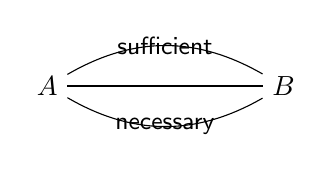
\begin{tikzpicture}
    \node[] (a) at (0,0) {$A$};
    \node[] (b) at (3,0) {$B$};
    \path[every node/.style={font=\sffamily\small}]
    (a) edge node {} (b)
    (b) edge[bend left] node {necessary} (a)
    (a) edge[bend left] node {sufficient} (b);
\end{tikzpicture}
\caption{The antecedent of a material conditional is a sufficient condition for the consequent, while the consequent is a necessary condition for the antecedent.}
\label{fig:necessary_and_sufficient}
\end{figure}


\section{Combining negation with conjunction and disjunction}

Tricky things happen when you combine a negation with a conjunction or disjunction, so it is worth taking a closer look here. Consider these sentences

\begin{description}
\item[\label{itm:or3}] Either you will not have soup, or you will not have salad.
\item[\label{itm:or4}] You will have neither soup nor salad.
\end{description}

We let $S_1$ mean that you get soup and $S_2$ mean that you get salad. Sentence \ref{itm:or3} can be paraphrased in this way: ``Either \emph{it is not the case that} you get soup, or \emph{it is not the case that} you get salad.'' Translating this requires both disjunction and negation. It becomes $\lnot S_1 \lor \lnot S_2$.

Sentence \ref{itm:or4} also requires negation. It can be paraphrased as, ``\emph{It is not the case that} either you get soup or you get salad.'' We need some way of indicating that the negation does not just negate the right or left disjunct, but rather negates the entire disjunction. In order to do this, we put parentheses around the disjunction: ``It is not the case that $(S_1 \lor S_2)$.'' This becomes simply $\lnot (S_1 \lor S_2)$. Notice that the parentheses are doing important work here. The sentence $\lnot S_1 \lor S_2$ would mean ``Either you will not have soup, or you will have salad.''

Something similar happens with negation and conjunction. Consider these sentences

\begin{description}
\item[\label{itm:notand1}] You can't have soup and you can't have salad.
\item[\label{itm:notand2}] You can't have both soup and salad.
\end{description}

In sentence \ref{itm:notand1}, the two parts of the sentence are negated individually. We would translate it into SL like this: $\lnot S_1 \land \lnot S_2$. In sentence \ref{itm:notand2}, the negation applies to soup and salad taken together. You are allowed to have soup only, or salad only. You just can't have both together. We would translate sentence \ref{itm:notand2} like this: $\lnot(S_1 \land S_2)$.

You can combine disjunction, conjunction, and negation to represent the exclusive or, as in this sentence.

\begin{description}
\item[\label{itm:or.xor}] You get either soup or salad, but not both.
\end{description}

Remember on page \pageref{def:inclusive_or}, we said that the $\lor$ in SL represented an inclusive or. It said ``this or that or both.'' If we want to represent an exclusive or, we need to combine disjunction, conjuction and negation. We can break the sentence into two parts. The first part says that you get one or the other. We translate this as $(S_1 \lor S_2)$. The second part says that you do not get both. We can paraphrase this as ``It is not the case both that you get soup and that you get salad.'' Using both negation and conjunction, we translate this as $\lnot(S_1 \land S_2)$. Now we just need to put the two parts together. As we saw above, ``but'' can usually be translated as a conjunction. Sentence \ref{itm:or.xor} can thus be translated as $(S_1 \lor S_2) \land \lnot(S_1 \land S_2)$.



\section{Recursive Syntax for SL}\label{recursive_syntax_for_SL}

The previous two sections gave you a rough, informal sense of how to create sentences in SL. If I give you an English sentence like ``Grass is either green or brown,'' you should be able to write a corresponding sentence in SL: ``$A \lor B$.'' In this section we want to give a more precise definition of a sentence in SL.  When we defined sentences in English, we did so using the concept of truth: Sentences were units of language that can be true or false. (See page \pageref{def:statement}.) In SL, it is possible to define what counts as a sentence without talking about truth. Instead, we can just talk about the structure of the sentence. This is one respect in which a formal language like SL is more precise than a natural language like English.

\newglossaryentry{syntax}
{
name=syntax,
description={The structure of a bit of language, considered without reference to truth, falsity, or meaning.}
}

\newglossaryentry{semantics}
{
name=semantics,
description={The meaning of a bit of language is its meaning, including truth and falsity.}
}

The structure of a sentence in SL considered without reference to truth or falsity is called its syntax. More generally \textsc{\gls{syntax}} \label{def:syntax} refers to the study of the properties of language that are there even when you don't consider meaning. Whether a sentence is true or false is considered part of its meaning. In this chapter, we will be giving a purely syntactical definition of a sentence in SL.  The contrasting term is \textsc{\gls{semantics}} \label{def:semantics} the study of aspects of language that relate to meaning, including truth and falsity. (The word ``semantics'' comes from the Greek word for ``mark'')

\newglossaryentry{object language}
{
name=object language,
description={A language that is constructed and studied by logicians. In this textbook, the object languages are SL and QL.
}


\newglossaryentry{metalanguage}
{
name=metalanguage,
description={The language logicians use to talk about the object language. In this textbook, the metalanguage is English, supplemented by certain symbols like metavariables and technical terms like ``valid.''}
}

If we are going to define a sentence in SL just using syntax, we will need to carefully distinguish SL from the language that we use to talk about SL. When you create an artificial language like SL, the language that you are creating is called the \textsc{\gls{object language}}. \label{def:object_language} The language that we use to talk about the object language is called the \textsc{\gls{metalanguage}}. \label{def:metalanguage} Imagine building a house. The object language is like the house itself. It is the thing we are building. While you are building a house, you might put up scaffolding around it. The scaffolding isn't part of the the house. You just use it to build the house. The metalanguage is like the scaffolding.

The object language in this chapter is SL. For the most part, we can build this language just by talking about it in ordinary English. However we will also have to build some special scaffolding that is not a part of SL, but will help us build SL. Our metalanguage will thus be ordinary English plus this scaffolding.

\newglossaryentry{metavariables}
{
name=metavariables,
description={A variable in the metalanguage that can represent any sentence in the object language.}
}

An important part of the scaffolding are the \textsc{\gls{metavariables}} \label{def:metavariables} These are the fancy script letters we have been using in the characteristic truth tables for the connectives: $\mathcal{A}$, $\mathcal{B}$, $\mathcal{C}$, etc. These are letters that can refer to any sentence in SL. They can represent sentences like $P$ or $Q$, or they can represent longer sentences, like $(((A \lor B) \land G) \onlyif (P \iff Q))$.
Just as the sentence letters $A$, $B$, etc. are variables that range over any English sentence, the metavariables $\mathcal{A}$, $\mathcal{B}$, etc. are variables that range over any sentence in SL, including the sentence letters $A$, $B$, etc.

As we said, in this chapter we will give a syntactic definition for ``sentence of SL.'' The definition itself will be given in mathematical English, the metalanguage. Table \ref{tab:basic_elements_of_SL} gives the basic elements of SL.


\begin{table}
\begin{tabu}{X[2] X[4]}
\textbf{Element} & \textbf{Symbols} \\
sentence letters & $A,B,C,\ldots,Z,A_1, B_1,Z_1,A_2,A_{25},J_{375},\ldots$ \\
connectives      & $\lnot,\land,\lor,\onlyif,\iff$ \\
parentheses      & $(,)$ \\
\end{tabu}
\caption{The basic elements of SL} \label{tab:basic_elements_of_SL}
\end{table}


Most random combinations of these symbols will not count as sentences in SL. Any random connection of these symbols will just be called a ``string'' or ``expression'' Random strings only become meaningful sentences when the are structured according to the rules of syntax. We saw from the earlier two sections that individual sentence letters,  like $A$ and $G_{13}$ counted as sentences. We also saw that we can put these sentences together using connectives so that  $\lnot A$ and $\lnot G_{13}$ is a sentence.  The problem is, we can't simply list all the different sentences we can put together this way, because there are infinitely many of them. Instead, we will define a sentence in SL by specifying the process by which they are constructed.

Consider negation: Given any sentence $\mathcal{A}$ of SL, $\lnot\mathcal{A}$ is a sentence of SL. It is important here that $\mathcal{A}$ is not the sentence letter $A$. Rather, it is a metavariable: part of the metalanguage, not the object language. Since $\mathcal{A}$ is not a symbol of SL, $\lnot\mathcal{A}$ is not an expression of SL. Instead, it is an expression of the metalanguage that allows us to talk about infinitely many expressions of SL: all of the expressions that start with the negation symbol.

\newglossaryentry{sentence of SL}
{
name=sentence of SL,
description={A string of symbols in SL that can be built up using according to the recursive rules given on page} % }
}

We can say similar things for each of the other connectives. For instance, if $\mathcal{A} and \mathcal{B}$ are sentences of SL, then $(\mathcal{A}\land\mathcal{B})$ is a sentence of SL. Providing clauses like this for all of the connectives, we arrive at the following formal definition for a \textsc{\gls{sentence of SL}}: \label{def:sentence_of_SL}

\begin{enumerate}
\item Every atomic sentence is a sentence.
\item If $\mathcal{A}$ is a sentence, then $\lnot\mathcal{A}$ is a sentence of SL.
\item If $\mathcal{A}$ and $\mathcal{B}$ are sentences, then $(\mathcal{A}\land\mathcal{B})$ is a sentence.
\item If $\mathcal{A}$ and $\mathcal{B}$ are sentences, then $(\mathcal{A}\lor\mathcal{B})$ is a sentence.
\item If $\mathcal{A}$ and $\mathcal{B}$ are sentences, then $(\mathcal{A}\onlyif\mathcal{B})$ is a sentence.
\item If $\mathcal{A}$ and $\mathcal{B}$ are sentences, then $(\mathcal{A}\iff\mathcal{B})$ is a sentence.
\item All and only sentences of SL can be generated by applications of these rules.
\end{enumerate}

We can apply this definition to see whether an arbitrary string is a sentence. Suppose we want to know whether or not $\lnot\lnot\lnot D$ is a sentence of SL.
Looking at the second clause of the definition, we know that $\lnot\lnot\lnot D$ is a sentence \emph{if} $\lnot\lnot D$ is a sentence.
So now we need to ask whether or not $\lnot\lnot D$ is a sentence.
Again looking at the second clause of the definition, $\lnot\lnot D$ is a sentence \emph{if} $\lnot D$ is.
Again, $\lnot D$ is a sentence \emph{if} $D$ is a sentence.
Now $D$ is a sentence letter, an atomic sentence of SL, so we know that $D$ is a sentence by the first clause of the definition.
So for a compound formula like $\lnot\lnot\lnot D$, we must apply the definition repeatedly. Eventually we arrive at the atomic sentences from which the sentence is built up.

\newglossaryentry{recursive definition}
{
name=recursive definition,
description={A definition that defines a term by identifying base class and rules for extending that class. Also called an ``inductive definition.''}
}

Definitions like this are called recursive. \textsc{\Glspl{recursive definition}}\label{def:recursive_definition} begin with some specifiable base elements and define ways to indefinitely compound the base elements. Just as the recursive definition allows complex sentences to be built up from simple parts, you can use it to decompose sentences into their simpler parts. To determine whether or not something meets the definition, you may have to refer back to the definition many times. Recursive definitions are also sometimes called ``inductive definitions.''

\newglossaryentry{sentential logic}
{
name=sentential logic,
description={A system of logic in which statements can be defined using a recursive definition with only sentences in the base class.}
}


We are now in a position to define what it means for a system of logic to be a system of sentential logic. A \textsc{\gls{sentential logic}} \label{def:sentential_logic} is a system of logic in which statements can be defined using a recursive definition with only sentences in the base class. This book defines on system of sentential logic, which we call SL. Other books use other systems.


\newglossaryentry{scope}
{
name=scope,
description={The sentences that are joined by a connective. These are the sentences the connective was applied to when the sentence was assembled using a recursive definition.}
}

When you use a connective to build a longer sentence from shorter ones, the shorter sentences are said to be in the \textsc{\gls{scope}} \label{def:scope} of the connective. So in the sentence $(A \land B) \onlyif C$, the scope of the connective $\onlyif$ includes $(A \land B)$ and C. In the sentence $\lnot(A \land B)$ the scope of the $\lnot$ is $(A \land B)$. On the other hand, in the sentence $\lnot A \land B$ the scope of the $\lnot$ is just $A$.

\newglossaryentry{main connective}
{
name=main connective,
description={The last connective that you add when you assemble a sentence using the recursive definition.}
}

The last connective that you add when you assemble a sentence using the recursive definition is the \textsc{\gls{main connective}} \label{def:main_connective} of that sentence. For example: The main logical operator of $\lnot (E \lor (F \onlyif G))$ is negation, $\lnot$. The main logical operator of $(\lnot E \lor (F \onlyif G))$ is disjunction, $\lor$. The main connective of any sentence will have all the rest of the sentence in its scope.

\newglossaryentry{unique readability}
{
name=unique readability,
description={A property of formal languages which is present when each well-formed formula is the product of a unique process of recursive construction.}
}

Because statement in our language is defined recursively, we can say it is ``uniquely readable.'' \textsc{\Gls{unique readability}}\label{def:unique_readability} is a property of formal languages which is present when each well-formed formula can only be constructed in a single way. Every process of building up a sentence recursively yields a unique sentence, and every sentence is the product of a unique process of recursive definitions. This means that in an important sense our language SL is free of ambiguity, which is a key goal in the construction of any formal language. Every sentence in SL will have a unambiguous main connective and every connective in a sentence will have an unambiguous scope. This makes logicians happy.


%The recursive structure of sentences in SL will be important when we consider the circumstances under which a particular sentence would be true or false. The sentence $\lnot $\lnot$ \lnot D$ is true if and only if the sentence $\lnot $\lnot$ D$ is false, and so on through the structure of the sentence until we arrive at the atomic components: $\lnot $\lnot$ \lnot D$ is true if and only if the atomic sentence $D$ is false. We will return to this point in the next chapter.
%restore when you restore the recursive part of chap. 3.

\section{Notational conventions}
\label{SLconventions}
A sentence like $(Q \land R)$ must be surrounded by parentheses, because we might apply the definition again to use this as part of a more complicated sentence. If we negate $(Q \land R)$, we get $\lnot(Q \land R)$. If we just had $Q \land R$ without the parentheses and put a negation in front of it, we would have $\lnot Q \land R$. It is most natural to read this as meaning the same thing as $(\lnot Q \land R)$, something very different than $\lnot(Q\land R)$. The sentence $\lnot(Q \land R)$ means that it is not the case that both $Q$ and $R$ are true; $Q$ might be false or $R$ might be false, but the sentence does not tell us which. The sentence $(\lnot Q \land R)$ means specifically that $Q$ is false and that $R$ is true. As such, parentheses are crucial to the meaning of the sentence.

So, strictly speaking, $Q \land R$ without parentheses is \emph{not} a sentence of SL. When using SL, however, we will often be able to relax the precise definition so as to make things easier for ourselves. We will do this in several ways.

First,  we understand that $Q \land R$ means the same thing as $(Q \land R)$. As a matter of convention, we can leave off parentheses that occur \emph{around the entire sentence}.

Second, it can sometimes be confusing to look at long sentences with many nested pairs of parentheses. We adopt the convention of using square brackets [ and ] in place of parentheses. There is no logical difference between $(P\lor Q)$ and $[P\lor Q]$, for example. The unwieldy sentence
$$(((H \onlyif I) \lor (I \onlyif H)) \land (J \lor K))$$
could be written in this way:
$$\bigl[(H \onlyif I) \lor (I \onlyif H)\bigr] \land (J \lor K)$$


Third, we will sometimes want to translate the conjunction of three or more sentences. For the sentence ``Alice, Bob, and Candice all went to the party,'' suppose we let $A$ mean ``Alice went,'' $B$ mean ``Bob went,'' and $C$ mean ``Candice went.'' The definition only allows us to form a conjunction out of two sentences, so we can translate it as $(A \land B) \land C$ or as $A \land (B \land C)$. There is no reason to distinguish between these, since the two translations are logically equivalent. There is no logical difference between the first, in which $(A \land B)$ is conjoined with $C$, and the second, in which $A$ is conjoined with $(B \land C)$.  So we might as well just write $A \land B \land C$. As a matter of convention, we can leave out parentheses when we conjoin three or more sentences.

Fourth, a similar situation arises with multiple disjunctions. ``Either Alice, Bob, or Candice went to the party'' can be translated as $(A \lor B) \lor C$ or as $A \lor (B \lor C)$. Since these two translations are logically equivalent, we may write $A \lor B \lor C$.

These latter two conventions only apply to multiple conjunctions or multiple  disjunctions. If a series of connectives includes both disjunctions and conjunctions, then the parentheses are essential; as with $(A \land B) \lor C$ and $A \land (B \lor C)$. The parentheses are also required if there is a series of conditionals or biconditionals; as with $(A \onlyif B) \onlyif C$ and $A \iff (B \iff C)$.

We have adopted these four rules as notational conventions, not as changes to the definition of a sentence. Strictly speaking, $A \lor B \lor C$ is still not a sentence. Instead, it is a kind of shorthand. We write it for the sake of convenience, but we really mean the sentence $(A \lor (B \lor C))$.

If we had given a different definition for a sentence, then these could count as sentences. We might have written rule 3 in this way: ``If $\mathcal{A}, \mathcal{B}, \ldots \mathcal{Z}$ are sentences, then $(\mathcal{A}\land\mathcal{B}\land\ldots\land\mathcal{Z})$, is a sentence .'' This would make it easier to translate some English sentences, but would have the cost of making our formal language more complicated. We would have to keep the complex definition in mind when we develop truth tables and a proof system. We want a logical language that is expressively simple and allows us to translate easily from English, but we also want a formally simple language. Adopting notational conventions is a compromise between these two desires.


\section*{Key Terms}
\begin{multicols}{2}
\begin{sortedlist}
\sortitem{Sentence letter}{}
\sortitem{Symbolization key}{}
\sortitem{Atomic sentence}{}
\sortitem{Sentential connective}{}
\sortitem{Negation}{}
\sortitem{Conjunction}{}
\sortitem{Conjunct}{}
\sortitem{Disjunction}{}
\sortitem{Disjunct}{}
\sortitem{Conditional}{}
\sortitem{Antecedent}{}
\sortitem{Consequent}{}
\sortitem{Biconditional}{}
\sortitem{Syntax}{}
\sortitem{Semantics}{}
\sortitem{Object language}{}
\sortitem{Metalanguage}{}
\sortitem{Metavariables}{}
\sortitem{Sentence of SL}{}
\sortitem{Main connective}{}
\sortitem{Recursive definition}{}
\sortitem{Scope}{}
\sortitem{Nonlogical symbol}{}
\sortitem{Logical constant}{}
\sortitem{Exclusive or}{}
\sortitem{Inclusive or}{}
\sortitem{Necessary condition}{}
\sortitem{Sufficient condition}{}
\sortitem{Translation key}{}
\end{sortedlist}
\end{multicols}
